\documentclass[journal]{IEEEtran}
\IEEEoverridecommandlockouts

\usepackage{cite}
\usepackage{amsmath,amssymb,amsfonts}
\usepackage{booktabs}
\usepackage{tabularx}
\usepackage{multirow}
\usepackage{graphicx}
\usepackage{textcomp}
\usepackage{xcolor}
\usepackage{url}
\usepackage{tikz}
\usepackage{pgfplots}
\pgfplotsset{compat=1.18}
\usetikzlibrary{arrows.meta,positioning,calc,shapes.geometric,
                decorations.pathreplacing,patterns}

%% ── colour palette ───────────────────────────────────────────────────────────
\definecolor{cblu} {RGB}{ 50,110,190}
\definecolor{cgrn} {RGB}{ 40,150, 70}
\definecolor{cora} {RGB}{210,110, 30}
\definecolor{cred} {RGB}{200, 50, 50}
\definecolor{cyel} {RGB}{190,165,  0}
\definecolor{cpur} {RGB}{130, 50,170}
\definecolor{cgry} {RGB}{100,100,100}

\begin{document}

\title{From Wire to Air: Security Limitations of EAP in Wireless 802.11 Environments and the Role of Outer Authentication via TLS Tunneling}

\author{Ezekiel~Ologunde,~\IEEEmembership{Independent~Researcher}
\thanks{E.\ Ologunde is an independent cybersecurity researcher. Email: ologunde@bu.edu}}

\markboth{IEEE Transactions on Information Forensics and Security}%
{Ologunde: EAP Security Limitations in Wireless 802.11 Environments}

\maketitle

\begin{abstract}
The Extensible Authentication Protocol (EAP), standardised in RFC~3748 and deployed
through IEEE~802.1X port-based network access control, was designed under the
assumption that the physical link between supplicant and authenticator is trusted.
This assumption is well-founded in wired Ethernet environments, where physical access
to the medium implies substantial prior authorisation. It collapses entirely in
IEEE~802.11 wireless networks, where the radio medium is inherently open and
accessible to any receiver within range. This paper provides a structured analysis of
the security limitations that emerge when EAP is deployed over 802.11, examining how
the open radio medium enables passive credential interception, rogue access point
impersonation, and replay attacks that the base EAP architecture offers no protection
against. We then analyse the two-phase authentication model introduced by tunnelled
EAP methods---PEAP, EAP-TTLS, and EAP-FAST---in which an outer authentication phase
establishes a TLS-protected tunnel via server-side digital certificate verification
before inner authentication credentials are exchanged. We demonstrate that this
layered architecture is not merely a performance optimisation but a structural
security requirement: without the TLS tunnel, inner authentication credentials are
transmitted in the clear over an open radio channel regardless of the cryptographic
strength of those credentials. The analysis evaluates PEAP, EAP-TTLS, and EAP-FAST
against this requirement, surveys common deployment vulnerabilities arising from
misconfigured certificate validation, and proposes a hardening framework for
enterprise wireless deployments.
\end{abstract}

\begin{IEEEkeywords}
EAP, 802.1X, 802.11, PEAP, EAP-TTLS, TLS tunnel, outer authentication, inner
authentication, wireless security, certificate validation, rogue access point
\end{IEEEkeywords}

%%─────────────────────────────────────────────────────────────────────────────
\section{Introduction}
%%─────────────────────────────────────────────────────────────────────────────

\IEEEPARstart{T}{he} Extensible Authentication Protocol (EAP), specified in
RFC~3748~\cite{rfc3748} and extended by RFC~5247~\cite{rfc5247}, was designed as a
flexible authentication framework for point-to-point links. Its earliest deployments
used it over Point-to-Point Protocol (PPP) connections for dial-up remote access,
and it was subsequently adopted as the authentication framework for IEEE~802.1X
port-based network access control~\cite{ieee8021x}. In both of these original
contexts, EAP operates over a link that is either physically secure (a serial cable,
a telco line) or administratively controlled (a switched Ethernet port behind a
physical lock). The EAP specification itself explicitly acknowledges this design
constraint, noting that it assumes a ``secured lower layer''~\cite{rfc3748}.

When 802.1X was extended to wireless 802.11 networks through the introduction of
WPA-Enterprise and WPA2-Enterprise modes~\cite{ieee80211i}, this assumption was
removed from the deployment environment while remaining present in the protocol
architecture. The result is a structural mismatch: EAP authentication exchanges
that were designed to run over trusted physical links are now broadcast over open
radio channels accessible to any receiver within range. This mismatch creates a
class of vulnerabilities---passive credential interception, rogue access point
attacks, and replay exploitation---that are absent from wired deployments and that
the base EAP protocol has no mechanism to address.

The response to this mismatch, developed over the period 2002--2007, is a family
of tunnelled EAP methods that introduce a two-phase authentication structure. The
first phase, known as outer authentication, establishes a TLS-protected tunnel
between the wireless client and the authentication server before any user credentials
are exchanged. The second phase, inner authentication, exchanges the actual user
credentials within the protection of that tunnel. This paper analyses both the
vulnerabilities that motivate this architecture and the architecture itself, with
particular attention to the role of digital certificates in making the outer
authentication phase security-meaningful.

\subsection{Contributions}

\begin{itemize}
  \item A formal analysis of the EAP security model and how the ``secured lower
        layer'' assumption fails in 802.11 environments
  \item An examination of the attack surface exposed by unprotected EAP over
        wireless, including passive interception, rogue AP attacks, and replay
  \item A technical analysis of the outer authentication / inner authentication
        architecture of PEAP, EAP-TTLS, and EAP-FAST
  \item An evaluation of why TLS with server-side certificate validation is a
        structural prerequisite for inner authentication security
  \item A survey of deployment vulnerabilities arising from misconfigured certificate
        validation and a hardening framework addressing them
\end{itemize}

%%─────────────────────────────────────────────────────────────────────────────
\section{EAP Architecture and the 802.1X Framework}
%%─────────────────────────────────────────────────────────────────────────────

\subsection{EAP Protocol Structure}

EAP is a lock-step request-response protocol in which the authenticator sends
\texttt{EAP-Request} messages and the supplicant responds with \texttt{EAP-Response}
messages. The protocol defines three principal roles~\cite{rfc3748}:

\begin{itemize}
  \item \textbf{Supplicant.} The network client seeking access. In enterprise wireless,
        this is the workstation, laptop, or mobile device.
  \item \textbf{Authenticator.} The device enforcing access control. In wired 802.1X
        this is the network switch; in wireless 802.1X this is the access point.
  \item \textbf{Authentication Server.} The back-end server that verifies credentials
        and makes access decisions. Typically a RADIUS server~\cite{rfc2865}
        implementing IEEE~802.1X.
\end{itemize}

Figure~\ref{fig:eap_arch} illustrates the three-role architecture and the
communication paths between them.

\begin{figure}[!t]
\centering
\scalebox{0.82}{
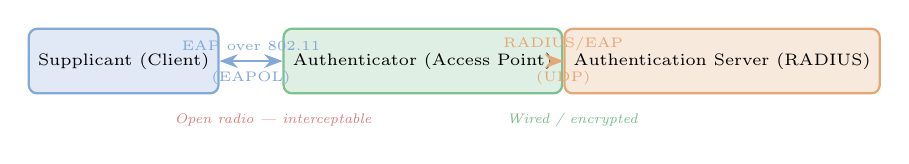
\begin{tikzpicture}[
  font=\fontsize{6.5pt}{8pt}\selectfont,
  >=Stealth,
  role/.style={rectangle, rounded corners=3pt, draw, thick,
               minimum width=2.2cm, minimum height=0.82cm, text centered},
  arr/.style={-{Stealth}, thick},
  dbl/.style={{Stealth}-{Stealth}, thick}
]
  \node[role, fill=cblu!15, draw=cblu!60] (SUP) at (0,   0) {Supplicant (Client)};
  \node[role, fill=cgrn!15, draw=cgrn!60] (AUTH) at (3.8, 0) {Authenticator (Access Point)};
  \node[role, fill=cora!15, draw=cora!60] (AS)  at (7.6, 0) {Authentication Server (RADIUS)};

  %% EAP over 802.11 / 802.1X
  \draw[dbl, cblu!60] (SUP.east) -- node[above,font=\fontsize{5.5pt}{7pt}\selectfont]
    {EAP over 802.11} node[below,font=\fontsize{5.5pt}{7pt}\selectfont]
    {(EAPOL)} (AUTH.west);

  %% RADIUS between authenticator and server
  \draw[dbl, cora!60] (AUTH.east) -- node[above,font=\fontsize{5.5pt}{7pt}\selectfont]
    {RADIUS/EAP} node[below,font=\fontsize{5.5pt}{7pt}\selectfont]
    {(UDP)} (AS.west);

  %% Labels below
  \node[font=\fontsize{5.5pt}{7pt}\selectfont\itshape, text=cred!65]
    at (1.9,-0.75) {Open radio --- interceptable};
  \node[font=\fontsize{5.5pt}{7pt}\selectfont\itshape, text=cgrn!65]
    at (5.7,-0.75) {Wired / encrypted};
\end{tikzpicture}
}% scalebox
\caption{IEEE 802.1X three-role architecture in a wireless deployment. The
  supplicant-to-authenticator segment runs over the open 802.11 radio medium;
  the authenticator-to-server segment is wired and optionally encrypted.}
\label{fig:eap_arch}
\end{figure}

EAP carries authentication data but does not itself provide confidentiality,
integrity, or replay protection for the authentication exchange. These properties
must be provided either by the lower-layer link (assumed secure in the original
design) or by an EAP method that establishes its own cryptographic
protection~\cite{rfc3748}.

\subsection{802.1X Port-Based Access Control}

IEEE~802.1X~\cite{ieee8021x} uses EAP as the authentication protocol for port-based
network access control. An 802.1X-enabled port begins in an \emph{unauthorised} state
that permits only EAP authentication traffic. Upon successful authentication, the
port transitions to an \emph{authorised} state granting full network access. In
wireless deployments, this model is implemented through EAPOL (EAP over LAN) messages
exchanged between the supplicant and access point.

The critical architectural property of 802.1X is that it performs authentication
before network access is granted. This is an important security control: an adversary
who cannot complete authentication cannot reach internal network resources. However,
this control only provides the intended protection if the authentication exchange
itself cannot be observed, replayed, or impersonated---properties that the 802.11
radio medium does not guarantee.

%%─────────────────────────────────────────────────────────────────────────────
\section{The Secured Lower Layer Assumption and Its Failure in 802.11}
%%─────────────────────────────────────────────────────────────────────────────

\subsection{Physical Security in Wired Environments}

In wired 802.1X deployments, the physical link between the supplicant and the
authenticating switch port is a point-to-point Ethernet segment---typically a
cable run from a wall jack to a workstation. The security model treats this segment
as trusted for two reasons. First, physical access to the cable or wall jack is
controlled by the physical security of the building: an adversary who can tap a
cable inside a secured facility has already defeated physical access controls whose
cost far exceeds the value of observing an authentication exchange. Second, switched
Ethernet does not broadcast traffic between arbitrary ports; even an adversary on
the same switched network segment cannot passively observe another station's
authentication traffic~\cite{edney2004}.

These conditions justify treating the lower layer as secured and, consequently,
treating the authentication exchange itself as having adequate confidentiality. A
lightweight EAP method that exchanges credentials in a form that would be easily
cracked if captured is nonetheless safe in practice because there is no practical
mechanism for capture.

\subsection{The 802.11 Radio Medium: An Open Broadcast Channel}

The wireless 802.11 medium does not share any of the properties that justify the
secured lower layer assumption. 802.11 is a shared broadcast medium: every frame
transmitted by any station is physically broadcast in all directions and is
receivable by any device with an appropriate radio within the coverage area. There
is no physical mechanism that restricts who can receive any given frame. The
802.11 specification provides no mandatory link-layer encryption for management
and authentication frames, and even when data-plane encryption (WEP, TKIP, CCMP)
is applied, it applies to data frames after association---not to the EAP
authentication frames exchanged during the association process~\cite{ieee80211i}.

The practical consequence is that every byte of an EAP authentication exchange
over 802.11 is transmitted in the clear to every receiver within radio range. An
adversary does not need physical proximity to the cable or wall jack; they need only
be within the access point's coverage area---typically tens to hundreds of metres
in open environments. This eliminates the physical access cost that makes cable
tapping impractical, reducing the cost of capturing an authentication exchange to
the purchase price of a commodity 802.11 network adapter~\cite{potter2005}.

\subsection{Attack Classes Enabled by the Open Radio Medium}

The exposure of EAP authentication traffic over the 802.11 medium enables three
primary attack classes, each with distinct mechanisms and impacts.

\subsubsection{Passive Credential Interception}

EAP methods that exchange credentials or credential-derived values in forms
susceptible to offline attack (e.g., MS-CHAPv2 challenge-response exchanges in
LEAP or unprotected MSCHAPv2) become trivially attackable when the exchange can be
passively captured. An adversary captures the EAP exchange using a standard wireless
frame capture tool, extracts the challenge and response values, and submits them to
an offline dictionary or brute-force attack. The ASLEAP attack against Cisco LEAP
demonstrated this class of vulnerability definitively in 2003, achieving credential
recovery from passive captures using dictionary attacks~\cite{wright2003asleap}.

\subsubsection{Rogue Access Point Impersonation}

The 802.11 association process does not include any mechanism for the supplicant to
verify the identity of the access point it is connecting to. An adversary can deploy
a rogue access point broadcasting the same SSID as the legitimate network, causing
clients to associate with the adversary's equipment instead of the legitimate
infrastructure. If the EAP authentication method does not include server-side
authentication (verification of the authenticator's identity by the supplicant), the
client will proceed to exchange credentials with the rogue access point, delivering
them directly to the adversary~\cite{arbaugh2002}.

\subsubsection{Replay and Man-in-the-Middle Attacks}

Without message authentication and replay protection in the EAP exchange,
an adversary who captures a successful authentication exchange may replay the
captured frames to gain access after the legitimate session has ended, or may insert
themselves as a transparent relay between supplicant and authenticator to observe
and modify the exchange in real time. While many EAP methods include
challenge-response mechanisms that prevent literal replay of authentication values,
the absence of link-layer integrity protection for EAP frames creates opportunities
for frame injection and manipulation~\cite{he2004}.

Figure~\ref{fig:attack_surface} maps these attack classes to the 802.11
EAP authentication flow.

\begin{figure*}[!t]
\centering
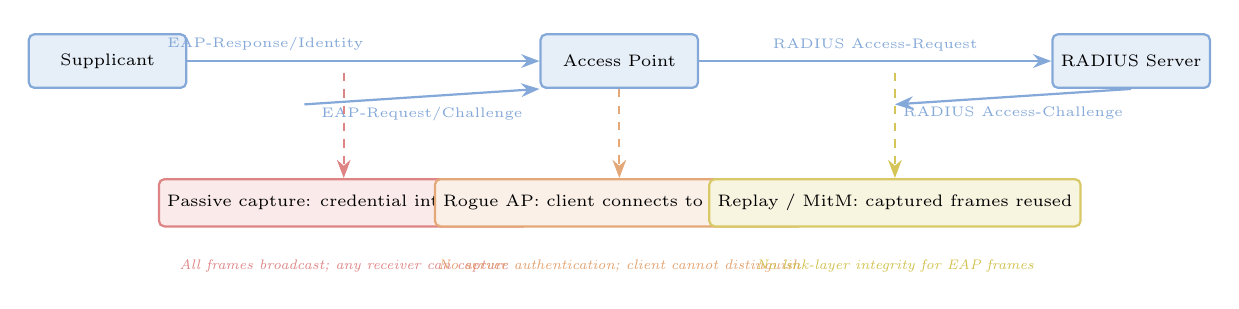
\begin{tikzpicture}[
  font=\fontsize{6.5pt}{8pt}\selectfont,
  >=Stealth,
  entity/.style={rectangle, rounded corners=2pt, draw=cblu!60, thick,
                 fill=cblu!12, minimum width=2.0cm, minimum height=0.68cm,
                 text centered, inner sep=3pt},
  atk/.style={rectangle, rounded corners=2pt, draw=cred!60, thick,
              fill=cred!10, minimum width=2.6cm, minimum height=0.60cm,
              text centered, font=\fontsize{6pt}{7.5pt}\selectfont, inner sep=3pt},
  msg/.style={-{Stealth}, thick, cblu!60},
  tap/.style={-{Stealth}, thick, dashed, cred!60}
]
  %% Entities
  \node[entity] (SUP) at (0,0) {Supplicant};
  \node[entity] (AP)  at (6.5,0) {Access Point};
  \node[entity] (AS)  at (13.0,0) {RADIUS Server};

  %% EAP exchange arrows
  \draw[msg] (SUP.east) -- node[above,font=\fontsize{5.5pt}{7pt}\selectfont]
    {EAP-Response/Identity} (3.0,0) -- (AP.west);
  \draw[msg] (AP.east) -- node[above,font=\fontsize{5.5pt}{7pt}\selectfont]
    {RADIUS Access-Request} (AS.west);
  \draw[{Stealth}-,msg] (2.5,-0.55) -- node[below,font=\fontsize{5.5pt}{7pt}\selectfont]
    {EAP-Request/Challenge} (AP.south west);
  \draw[{Stealth}-,msg] (AS.south) -- node[below,font=\fontsize{5.5pt}{7pt}\selectfont]
    {RADIUS Access-Challenge} (10.0,-0.55);

  %% Attack 1: passive capture
  \node[atk] (A1) at (3.0,-1.80) {Passive capture: credential interception};
  \draw[tap] (3.0,-0.15) -- (A1.north);
  \node[font=\fontsize{5.5pt}{7pt}\selectfont\itshape, text=cred!60]
    at (3.0,-2.60) {All frames broadcast; any receiver can capture};

  %% Attack 2: rogue AP
  \node[atk, fill=cora!10, draw=cora!60] (A2) at (6.5,-1.80)
    {Rogue AP: client connects to adversary};
  \draw[tap, cora!60] (AP.south) -- (A2.north);
  \node[font=\fontsize{5.5pt}{7pt}\selectfont\itshape, text=cora!65]
    at (6.5,-2.60) {No server authentication; client cannot distinguish};

  %% Attack 3: replay / MitM
  \node[atk, fill=cyel!12, draw=cyel!60] (A3) at (10.0,-1.80)
    {Replay / MitM: captured frames reused};
  \draw[tap, cyel!65] (10.0,-0.15) -- (A3.north);
  \node[font=\fontsize{5.5pt}{7pt}\selectfont\itshape, text=cyel!70]
    at (10.0,-2.60) {No link-layer integrity for EAP frames};
\end{tikzpicture}
\caption{Attack surface exposed by unprotected EAP authentication over 802.11.
  Passive capture, rogue access point impersonation, and replay/MitM attacks all
  exploit the absence of channel confidentiality and server authentication in base
  EAP~\cite{arbaugh2002,wright2003asleap,he2004}.}
\label{fig:attack_surface}
\end{figure*}

%%─────────────────────────────────────────────────────────────────────────────
\section{Outer Authentication: Establishing a TLS Secure Tunnel}
%%─────────────────────────────────────────────────────────────────────────────

\subsection{The Two-Phase Authentication Model}

The solution to the vulnerabilities described in Section~III is a two-phase
authentication model in which a \emph{secure channel} is established before any
sensitive credentials are exchanged. This model is implemented by a family of
tunnelled EAP methods: Protected EAP (PEAP)~\cite{peap}, EAP Tunneled TLS
(EAP-TTLS)~\cite{rfc5281}, and EAP Flexible Authentication via Secure Tunneling
(EAP-FAST)~\cite{rfc4851}. All three share the same architectural principle: a
two-phase exchange consisting of outer authentication followed by inner
authentication.

\textbf{Outer authentication} establishes a TLS secure tunnel between the wireless
client and the authentication server. This phase is analogous to the TLS handshake
in HTTPS: the authentication server presents a digital certificate that the client
can verify, the two parties negotiate cryptographic parameters, and a shared session
key is established. The output of outer authentication is an encrypted channel that
protects all subsequent communication.

\textbf{Inner authentication} occurs entirely within the TLS tunnel established in
the outer phase. The client presents its actual credentials---username and password,
an MS-CHAPv2 exchange, or a client-side digital certificate---and the authentication
server validates them. Because this exchange occurs inside the TLS tunnel, it is
encrypted and cannot be observed or manipulated by an adversary on the radio medium.

Figure~\ref{fig:two_phase} illustrates the two-phase authentication exchange in
the PEAP case.

\begin{figure}[!t]
\centering
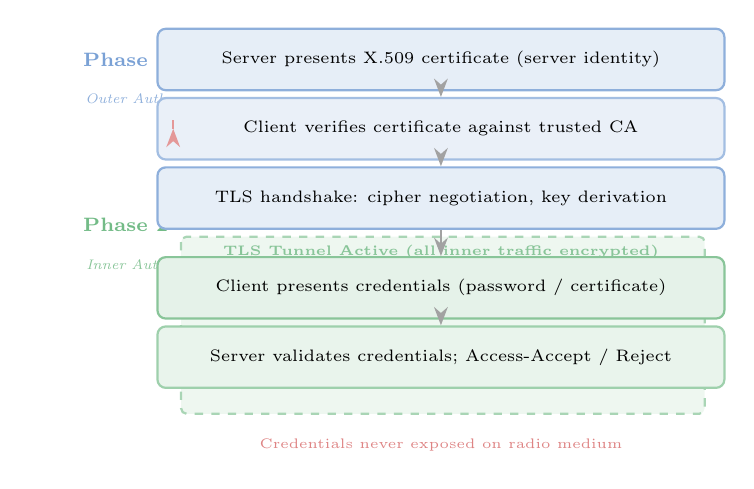
\begin{tikzpicture}[
  font=\fontsize{6.5pt}{8pt}\selectfont,
  >=Stealth,
  phase/.style={rectangle, rounded corners=3pt, draw, thick,
                minimum width=7.2cm, minimum height=0.78cm,
                text centered, inner sep=3pt},
  arr/.style={-{Stealth}, thick, cgry!60}
]
  %% Phase labels on left
  \node[font=\fontsize{7pt}{9pt}\selectfont\bfseries, text=cblu!65]
    at (-0.8,0) {Phase 1};
  \node[font=\fontsize{5.5pt}{7pt}\selectfont\itshape, text=cblu!55]
    at (-0.8,-0.50) {Outer Auth};

  \node[font=\fontsize{7pt}{9pt}\selectfont\bfseries, text=cgrn!65]
    at (-0.8,-2.10) {Phase 2};
  \node[font=\fontsize{5.5pt}{7pt}\selectfont\itshape, text=cgrn!55]
    at (-0.8,-2.60) {Inner Auth};

  %% Outer phase steps
  \node[phase, fill=cblu!12, draw=cblu!55] (p11) at (3.2, 0.00)
    {Server presents X.509 certificate (server identity)};
  \node[phase, fill=cblu!10, draw=cblu!45] (p12) at (3.2,-0.88)
    {Client verifies certificate against trusted CA};
  \node[phase, fill=cblu!12, draw=cblu!55] (p13) at (3.2,-1.76)
    {TLS handshake: cipher negotiation, key derivation};

  %% Tunnel established marker
  \filldraw[fill=cgrn!8, draw=cgrn!40, thick, rounded corners=2pt, dashed]
    (-0.1,-2.25) rectangle (6.55,-4.50);
  \node[font=\fontsize{5.5pt}{7pt}\selectfont\bfseries, text=cgrn!55]
    at (3.2,-2.45) {TLS Tunnel Active (all inner traffic encrypted)};

  %% Inner phase steps
  \node[phase, fill=cgrn!12, draw=cgrn!55] (p21) at (3.2,-2.90)
    {Client presents credentials (password / certificate)};
  \node[phase, fill=cgrn!10, draw=cgrn!45] (p22) at (3.2,-3.78)
    {Server validates credentials; Access-Accept / Reject};

  \draw[arr] (p11)--(p12); \draw[arr] (p12)--(p13);
  \draw[arr] (p13)--(p21); \draw[arr] (p21)--(p22);

  \draw[-{Stealth}, cred!50, thick, dashed] (-0.2,-0.88) -- (-0.2,-0.88)
    node[left, font=\fontsize{5.5pt}{7pt}\selectfont, text=cred!60, align=right,
         text width=1.6cm] {};
  \node[font=\fontsize{5.5pt}{7pt}\selectfont, text=cred!60, align=center]
    at (3.2,-4.90) {Credentials never exposed on radio medium};
\end{tikzpicture}
\caption{Two-phase PEAP authentication exchange. The outer authentication phase
  (Phase~1) establishes a TLS tunnel through server certificate verification.
  Inner authentication credentials (Phase~2) are exchanged exclusively within
  the encrypted tunnel.}
\label{fig:two_phase}
\end{figure}

\subsection{Why Digital Certificates Are a Prerequisite}

The TLS tunnel established during outer authentication provides confidentiality and
integrity for the inner authentication exchange. However, a TLS tunnel alone is not
sufficient to provide security unless the client can verify that it is communicating
with the legitimate authentication server rather than with an adversary's rogue
access point. This verification is the role of the server-side digital certificate.

A digital certificate~\cite{rfc5280} is a cryptographically signed data structure
that binds a public key to an identity (the authentication server's hostname or
other identifier) and is signed by a Certificate Authority (CA) trusted by the
client. During the outer authentication TLS handshake, the authentication server
presents its certificate, and the client performs the following verification
operations:

\begin{enumerate}
  \item \textbf{Certificate chain validation.} The client verifies that the
        server's certificate is signed by a CA whose certificate appears in the
        client's trust store.
  \item \textbf{Certificate validity.} The client checks that the certificate has
        not expired and has not been revoked.
  \item \textbf{Server identity verification.} The client checks that the identity
        asserted in the certificate (typically the RADIUS server's fully qualified
        domain name) matches the expected authentication server for the network
        being joined.
  \item \textbf{Proof of possession.} The TLS handshake includes a challenge-response
        step in which the server proves it possesses the private key corresponding
        to the public key in the certificate, preventing certificate copying attacks.
\end{enumerate}

If any of these verification steps fails, the client should abort the connection.
The critical point is that only step~1 (certificate chain validation to a trusted CA)
can be automated by the client software; steps~3 and~4 require that the client be
correctly configured with the expected server identity and that the server actually
possesses the private key. If the client skips step~3---a misconfiguration common
in enterprise deployments~\cite{asokan2013}---a rogue access point can present any
certificate signed by a CA in the client's trust store (which for devices using the
OS default trust store includes hundreds of commercial CAs) and the client will
proceed to exchange inner authentication credentials with the adversary.

\subsection{The Certificate Validation Gap: A Critical Deployment Vulnerability}

The requirement for correct certificate validation highlights a gap between the
theoretical security of tunnelled EAP methods and their security as typically
deployed. The theoretical security model requires clients to verify the server's
certificate against a specifically configured internal CA and to verify the server
identity field. In practice, many enterprise deployments leave client devices
configured with either no certificate validation (explicitly disabled for
troubleshooting and never re-enabled), or validation against the full OS default
trust store without specifying the expected server identity~\cite{asokan2013}.

In either case, the rogue access point attack described in Section~III-B remains
fully viable: the adversary obtains a certificate from any commercial CA (a
straightforward process), deploys a rogue access point and RADIUS server, and
waits for clients to connect. Clients configured without proper certificate
validation complete the outer authentication phase with the adversary's server,
establishing a TLS tunnel to an adversary-controlled endpoint, and then
deliver their inner authentication credentials directly into the adversary's
RADIUS server.

This vulnerability is so prevalent that Asokan et al.~\cite{asokan2013} documented
it systematically in enterprise deployments and proposed the \emph{channel binding}
mechanism (RFC~6677~\cite{rfc6677}) as a cryptographic countermeasure, binding the
inner authentication exchange to the specific TLS channel in which it occurs to
prevent credential forwarding across distinct sessions.

%%─────────────────────────────────────────────────────────────────────────────
\section{Tunnelled EAP Methods: PEAP, EAP-TTLS, and EAP-FAST}
%%─────────────────────────────────────────────────────────────────────────────

\subsection{Protected EAP (PEAP)}

PEAP was developed jointly by Microsoft, Cisco, and RSA Security and is the most
widely deployed tunnelled EAP method in Microsoft Windows environments~\cite{peap}.
PEAP outer authentication uses TLS with mandatory server-side certificate presentation;
the client is not required to present a certificate during the outer phase. The
TLS tunnel thus provides server authentication (preventing rogue AP attacks) and
channel confidentiality (preventing passive capture of inner authentication traffic).

Within the PEAP tunnel, the inner authentication method is itself an EAP method.
The most common choice is PEAPv0/EAP-MSCHAPv2, in which the client authenticates
using a username and NT hash-derived challenge-response~\cite{peap}. The security
of this inner method depends entirely on the TLS tunnel: MSCHAPv2 in isolation is
vulnerable to offline dictionary attacks given captured exchanges, but inside the
PEAP tunnel those exchanges are not capturable by a passive adversary.

An alternative PEAP inner method is PEAPv1/EAP-GTC (Generic Token Card), which
supports one-time password tokens and is preferred in environments where password
reuse or dictionary attack risk is a primary concern.

\subsection{EAP Tunneled TLS (EAP-TTLS)}

EAP-TTLS~\cite{rfc5281} extends the PEAP architecture by supporting non-EAP inner
authentication methods within the TLS tunnel. Where PEAP requires the inner method
to be an EAP method, EAP-TTLS supports RADIUS attribute-based authentication,
allowing inner methods including PAP, CHAP, MS-CHAP, and MS-CHAPv2 to be used inside
the tunnel. This flexibility is valuable in environments with heterogeneous
authentication infrastructure, particularly where legacy systems support only specific
inner methods.

EAP-TTLS is more common in Linux and macOS environments and in deployments based on
FreeRADIUS or other open-source RADIUS implementations. Its inner method flexibility
comes with a corresponding requirement for careful inner method selection: PAP inside
an EAP-TTLS tunnel is secure against passive radio-side capture (because the tunnel
encrypts it) but transmits the password in plaintext to the RADIUS server,
introducing plaintext credential exposure at the server rather than the radio medium.

\subsection{EAP Flexible Authentication via Secure Tunneling (EAP-FAST)}

EAP-FAST~\cite{rfc4851} was developed by Cisco as an alternative to PEAP that
avoids the operational dependency on digital certificates for outer authentication.
Instead of TLS with a certificate, EAP-FAST outer authentication uses a
\emph{Protected Access Credential} (PAC)---a pre-provisioned shared secret that
provides the authenticated key establishment for the outer tunnel. PAC provisioning
can occur either out-of-band (PAC distributed to clients by an administrator) or
in-band through anonymous TLS during an initial provisioning exchange.

The security trade-off of EAP-FAST is that it replaces the asymmetric trust anchor
of a CA-issued certificate with a symmetric shared secret. This eliminates the
operational complexity of certificate management but introduces PAC management
complexity and creates a different attack surface: an adversary who obtains a client's
PAC can impersonate the authentication server for that client. The anonymous
provisioning mode, while operationally convenient, is vulnerable to a rogue server
intercepting the provisioning exchange and delivering a malicious PAC~\cite{rfc4851}.

Table~\ref{tab:tunneled_methods} provides a comparative summary of the three methods.

\begin{table}[!t]
\caption{Comparison of Tunnelled EAP Methods}
\label{tab:tunneled_methods}
\centering
\resizebox{\columnwidth}{!}{\begin{tabular}{@{}p{1.8cm}p{1.8cm}p{1.8cm}p{2.0cm}@{}}
\toprule
\textbf{Property} & \textbf{PEAP} & \textbf{EAP-TTLS} & \textbf{EAP-FAST} \\
\midrule
Outer auth   & TLS + server cert & TLS + server cert & TLS + PAC \\
Client cert required & No & No & No \\
Inner methods & EAP only & EAP + RADIUS attrs & EAP \\
Certificate dependency & High & High & Low \\
Rogue AP protection & Yes (if cert validation correct) & Yes (if cert validation correct) & Yes (if PAC valid) \\
Common platforms & Windows & Linux/macOS & Cisco \\
Standardisation & IETF Draft & RFC 5281 & RFC 4851 \\
\bottomrule
\end{tabular}}
\end{table}

%%─────────────────────────────────────────────────────────────────────────────
\section{The Layered Security Architecture: Why the Order Matters}
%%─────────────────────────────────────────────────────────────────────────────

\subsection{The Separation of Channel Security from Authentication}

The two-phase outer/inner authentication architecture embodies a fundamental
principle of security protocol design: the properties of the communication channel
and the properties of the authentication mechanism are separate concerns that must
be addressed independently. A strong authentication method (one whose credentials
cannot be easily forged) does not provide security if the credentials are observable
in transit; conversely, a confidential channel does not help if the server at the
other end cannot be verified as legitimate.

The outer authentication phase addresses the channel and the server identity
simultaneously: the TLS handshake establishes channel confidentiality and integrity,
and the certificate verification establishes the server's authenticated identity.
Only once both properties are established is it safe to proceed with inner
authentication. This ordering is not optional---it is structurally necessary.

If inner authentication were attempted before the TLS tunnel were established,
the credentials would be transmitted over the open 802.11 radio medium regardless
of how strong they are. An adversary who captures the exchange and submits the
credentials to an offline attack has bypassed whatever security the inner method
was designed to provide. The entire security of the inner authentication is
contingent on the tunnel being in place when inner authentication occurs.

\subsection{The Trust Anchor Requirement}

The TLS tunnel established during outer authentication provides genuine security
only if the certificate verification produces a meaningful trust decision. A TLS
tunnel with an unverified or incorrectly verified certificate is cryptographically
sound (the tunnel is encrypted and the server's private key is authenticated within
the session) but semantically empty: the client has established a secure channel
to an unknown destination. For a rogue access point, ``unknown destination'' is
precisely the adversary's server.

The trust anchor is the CA whose certificate the client has explicitly configured
as trusted for authenticating the specific network's authentication server. This
is distinct from general-purpose web browser trust stores, which include hundreds
of commercial CAs authorised to issue certificates for arbitrary domains. Enterprise
wireless authentication requires a narrow trust anchor: ideally the organisation's
own internal CA, configured on client devices through enterprise mobile device
management (MDM), with the specific RADIUS server hostname or IP address range
specified as the expected server identity.

\subsection{Certificate Validation as a Non-Negotiable Requirement}

Given the analysis above, it follows that server-side certificate validation---
specifically, validation against a purpose-specific trust anchor with server identity
checking---is a non-negotiable requirement for the outer authentication phase to
provide its intended security property. This requirement is frequently characterised
as a deployment complexity or a user experience burden (requiring MDM configuration
or user interaction with certificate warnings), but these characterisations conflate
operational convenience with security necessity. Disabling certificate validation
for operational simplicity creates an environment in which the tunnelled EAP
deployment provides the appearance of strong authentication while retaining all the
vulnerabilities of unprotected EAP~\cite{asokan2013}.

%%─────────────────────────────────────────────────────────────────────────────
\section{Practical Hardening Framework}
%%─────────────────────────────────────────────────────────────────────────────

\subsection{Certificate Management}

Effective outer authentication security requires a certificate management
infrastructure that provides the following:

\begin{itemize}
  \item \textbf{Internal CA.} An organisation-operated CA whose certificate is
        distributed to client devices through MDM or Group Policy. This restricts
        the set of valid RADIUS server certificates to those issued by the
        organisation, preventing commercial CA abuse.
  \item \textbf{Server identity pinning.} Client EAP profiles must specify the
        expected RADIUS server hostname or certificate hash, preventing acceptance
        of certificates from the correct CA but for an unexpected host.
  \item \textbf{Certificate lifecycle management.} RADIUS server certificates
        must be renewed before expiration; expired certificates will cause
        authentication failures if clients enforce validity checking.
  \item \textbf{Revocation checking.} Where feasible, OCSP or CRL-based revocation
        checking should be enabled to allow compromised certificates to be
        immediately invalidated.
\end{itemize}

\subsection{Client Profile Deployment}

Client 802.1X authentication profiles should be deployed through automated
mechanisms (MDM, Group Policy, JAMF, Intune) rather than manual configuration.
Manual configuration is error-prone and inconsistent; it is the primary cause of
the certificate validation gaps documented in Section~IV-C. Automated profile
deployment ensures that all clients have:

\begin{itemize}
  \item Certificate validation enabled
  \item The internal CA certificate installed in the appropriate trust store
  \item The expected RADIUS server identity configured
  \item The correct EAP type and inner method selected
\end{itemize}

\subsection{RADIUS Server Hardening}

The RADIUS authentication server is the trust anchor of the 802.1X deployment and
must be hardened accordingly:

\begin{itemize}
  \item TLS 1.2 minimum; TLS 1.3 preferred for all EAP-TLS connections
  \item Strong cipher suites with forward secrecy (ECDHE key exchange)
  \item Certificate key size of at least 2048-bit RSA or 256-bit ECDSA
  \item Network isolation of the RADIUS server from general-purpose network traffic
  \item Audit logging of all authentication events (success, failure, and
        certificate validation errors)
\end{itemize}

\subsection{Monitoring for Rogue Access Points}

Even with correctly deployed tunnelled EAP, rogue access point attacks can succeed
against clients with misconfigured profiles. Wireless intrusion detection systems
(WIDS) should be deployed to detect and alert on:

\begin{itemize}
  \item Access points broadcasting the enterprise SSID from unrecognised MAC addresses
  \item Authentication failures indicative of certificate validation errors
  \item Clients performing EAP exchanges with unrecognised BSSIDs
\end{itemize}

Table~\ref{tab:hardening} summarises the hardening framework.

\begin{table}[!t]
\caption{Enterprise Wireless EAP Hardening Framework}
\label{tab:hardening}
\centering
\resizebox{\columnwidth}{!}{\begin{tabular}{@{}p{2.5cm}p{5.5cm}p{2.5cm}@{}}
\toprule
\textbf{Control} & \textbf{Description} & \textbf{Addresses} \\
\midrule
Internal CA deployment & Client trust restricted to org CA; distributed via MDM & Rogue AP / cert abuse \\
Server identity pinning & Expected RADIUS hostname in client profiles & Rogue AP with valid cert \\
Cert lifecycle mgmt & Renewal before expiry; revocation checking & Expired/compromised certs \\
Automated profile push & MDM/GP deploys EAP profiles; no manual config & Misconfiguration \\
TLS 1.2+ RADIUS & Strong TLS; ECDHE; 2048-bit+ keys & Channel confidentiality \\
WIDS monitoring & Rogue SSID detection; auth failure alerting & Rogue AP detection \\
Channel binding (RFC 6677) & Binds inner auth to specific TLS session & Credential forwarding \\
\bottomrule
\end{tabular}}
\end{table}

%%─────────────────────────────────────────────────────────────────────────────
\section{Discussion}
%%─────────────────────────────────────────────────────────────────────────────

\subsection{The Fundamental Design Tension}

The analysis in this paper reveals a fundamental design tension in applying 802.1X
to wireless environments. The 802.1X framework was designed for a threat model in
which the lower layer is trusted; tunnelled EAP methods add an upper-layer security
mechanism to compensate for an untrusted lower layer. This is a form of security
retrofitting, and retrofitting generally produces weaker and more operationally
complex solutions than security architectures designed from the ground up for their
threat model.

The specific expression of this tension is the certificate validation problem:
the outer authentication phase provides its security guarantee only if correctly
deployed, but correct deployment requires organisational processes (internal CA
operation, MDM management, certificate lifecycle management) that are operationally
demanding. Organisations that cannot sustain these processes default to
configurations that silently remove the security property while preserving the
appearance of strong authentication.

\subsection{Alternatives and Complements}

Enterprise wireless security is not limited to 802.1X and tunnelled EAP. Mutual
certificate-based authentication through EAP-TLS (in which the client also presents
a certificate during the outer authentication phase) eliminates the inner
authentication phase entirely and provides stronger authentication guarantees:
credential interception is impossible because there are no credentials to
intercept~\cite{rfc5216}. However, EAP-TLS requires client certificate provisioning,
which is operationally comparable in complexity to the RADIUS server certificate
management already required.

WPA3-Enterprise with 192-bit security mode~\cite{wpa3} mandates stronger cipher
suites and certificate requirements and is increasingly the appropriate baseline
for new enterprise wireless deployments. Wi-Fi Enhanced Open (OWE)~\cite{rfc8110}
provides opportunistic wireless encryption for open networks but does not provide
authentication and is therefore not a substitute for 802.1X.

\subsection{The Security Proof for the Two-Phase Model}

The two-phase outer/inner authentication model provides a formal security
reduction: the security of the inner authentication against passive radio-side
observation reduces to the security of the TLS tunnel, which reduces to the
security of the TLS protocol and the correctness of the certificate verification.
If TLS is secure (as it is, under standard computational assumptions, for
correctly implemented TLS~1.3~\cite{rfc8446}) and certificate verification is
correct, then inner authentication credentials are informationally hidden from
any adversary on the radio medium. This is the sense in which outer authentication
is a \emph{prerequisite}: removing it removes the only mechanism by which the
inner authentication exchange is protected.

%%─────────────────────────────────────────────────────────────────────────────
\section{Conclusion}
%%─────────────────────────────────────────────────────────────────────────────

The Extensible Authentication Protocol exposes a class of security vulnerabilities
when deployed over wireless 802.11 networks that are absent from its original wired
deployment context. These vulnerabilities---passive credential interception, rogue
access point impersonation, and replay attacks---arise directly from the replacement
of a trusted physical medium with an inherently open radio channel, which eliminates
the ``secured lower layer'' assumption on which base EAP's security model depends.

Tunnelled EAP methods address these vulnerabilities through a two-phase
outer/inner authentication architecture. The outer authentication phase establishes
a TLS-protected channel using a server-side digital certificate, simultaneously
providing channel confidentiality and authenticated server identity. The inner
authentication phase exchanges user credentials exclusively within this protected
channel. The two phases are inseparable from a security perspective: inner
authentication credentials exposed on the radio medium are subject to all the attacks
that outer authentication is designed to prevent, regardless of the cryptographic
strength of the inner method.

The practical deployment challenge is ensuring that outer authentication's certificate
validation is correctly configured. Certificate validation failures---whether through
explicit disablement, misconfigured trust anchors, or absent server identity
checking---silently return the deployment to the vulnerability baseline of unprotected
EAP. Addressing this requires organisational investment in internal CA operation,
automated profile deployment through MDM, and continuous monitoring for rogue access
points and certificate validation anomalies. These operational requirements are the
non-negotiable cost of deploying EAP-based authentication securely in an inherently
open radio environment.

\section*{Acknowledgment}

The author acknowledges the foundational contributions of the IEEE 802.11i working
group, the IETF EAP and RADEXT working groups, and the security researchers whose
analysis of deployed tunnelled EAP vulnerabilities has driven the successive
improvements documented in this paper.

\sloppy
\bibliographystyle{IEEEtran}
\begin{thebibliography}{25}

\bibitem{rfc3748}
B.~Aboba, L.~Blunk, J.~Vollbrecht, J.~Carlson, and H.~Levkowetz.
2004. \textit{RFC 3748: Extensible Authentication Protocol (EAP)}.
IETF.

\bibitem{rfc5247}
B.~Aboba, D.~Simon, and P.~Eronen.
2008. \textit{RFC 5247: Extensible Authentication Protocol (EAP) Key Management Framework}.
IETF.

\bibitem{ieee8021x}
IEEE.
2020. \textit{IEEE Standard 802.1X-2020: Port-Based Network Access Control}.
IEEE.

\bibitem{ieee80211i}
IEEE.
2004. \textit{IEEE Standard 802.11i-2004: Medium Access Control Security Enhancements}.
IEEE.

\bibitem{rfc2865}
C.~Rigney, S.~Willens, A.~Rubens, and W.~Simpson.
2000. \textit{RFC 2865: Remote Authentication Dial In User Service (RADIUS)}.
IETF.

\bibitem{peap}
A.~Palekar, D.~Simon, G.~Zorn, N.~Salowey, H.~Zhou, and G.~Dommety.
2004. Protected EAP Protocol (PEAP). IETF Draft
\texttt{draft-josefsson-pppext-eap-tls-eap-10}.

\bibitem{rfc5281}
P.~Funk and S.~Blake-Wilson.
2008. \textit{RFC 5281: Extensible Authentication Protocol Tunneled Transport Layer Security Authenticated Protocol Version 0 (EAP-TTLSv0)}.
IETF.

\bibitem{rfc4851}
N.~Cam-Winget, D.~McGrew, J.~Salowey, and H.~Zhou.
2007. \textit{RFC 4851: The Flexible Authentication via Secure Tunneling Extensible Authentication Protocol Method (EAP-FAST)}.
IETF.

\bibitem{rfc5280}
D.~Cooper, S.~Santesson, S.~Farrell, S.~Boeyen, R.~Housley, and W.~Polk.
2008. \textit{RFC 5280: Internet X.509 Public Key Infrastructure Certificate and Certificate Revocation List (CRL) Profile}.
IETF.

\bibitem{rfc5216}
D.~Simon, B.~Aboba, and R.~Hurst.
2008. \textit{RFC 5216: The EAP-TLS Authentication Protocol}.
IETF.

\bibitem{rfc6677}
S.~Hartman, T.~Clancy, and K.~Hoeper.
2012. \textit{RFC 6677: Channel-Binding Support for Extensible Authentication Protocol Methods}.
IETF.

\bibitem{rfc8446}
E.~Rescorla.
2018. \textit{RFC 8446: The Transport Layer Security (TLS) Protocol Version 1.3}.
IETF.

\bibitem{rfc8110}
D.~Harkins and W.~Kumari.
2017. \textit{RFC 8110: Opportunistic Wireless Encryption}.
IETF.

\bibitem{arbaugh2002}
W.~A.~Arbaugh, N.~Shankar, Y.~C.~J.~Wan, and K.~Zhang.
2002. Your 802.11 Wireless Network Has No Clothes.
\textit{IEEE Wireless Communications}, vol.~9, no.~6, pp.~44--51.

\bibitem{wright2003asleap}
J.~Wright.
2003. Defining a New Active Attack Against LEAP Authentication.
\textit{Network World}. Available: \url{https://www.willhackforsushi.com/Leaflet.pdf}

\bibitem{he2004}
C.~He and J.~C.~Mitchell.
2004. Security Analysis and Improvements for IEEE 802.11i.
In \textit{Proc.\ 11th Annual Network and Distributed System Security Symposium
(NDSS~2004)}.

\bibitem{asokan2013}
N.~Asokan, T.~Elo, K.~Kostiainen, A.~Lentz, J.-P.~Seifert, and E.~Trichina.
2013. Mobile Terminal Security.
In \textit{Proc.\ ACM CCS 2013}.

\bibitem{edney2004}
J.~Edney and W.~A.~Arbaugh.
2004. \textit{Real 802.11 Security: Wi-Fi Protected Access and 802.11i}.
Addison-Wesley.

\bibitem{potter2005}
B.~Potter and G.~McGraw.
2005. Wireless Security's Evolution.
\textit{IEEE Security \& Privacy}, vol.~3, no.~2, pp.~65--68.

\bibitem{wpa3}
Wi-Fi Alliance.
2019. \textit{Wi-Fi CERTIFIED WPA3 Specification, Version 1.0}.
Wi-Fi Alliance.

\end{thebibliography}

\end{document}
